\section{Gruppetype}
\label{sec:gruppetype}
Det er uten tvil svært stort spenn i gruppers effektivitet og produktivitet. Johnson \& Johnson (2013) \citep{gruppeteori} har delt grupper inn i fire typer basert på effektivitet som illustrert i figur \ref{fig:gruppetype}:
\begin{enumerate}
\item \textit{Pseudogrupper:} medlemmer er tilordnet arbeid i en gruppe uten å ha noe interesse av å gjøre dette. Medlemmer ser hverandre som konkurrenter fremfor samarbeidspartnere og summen av gruppearbeidet tilsvarer derfor mindre enn summen av potensialet til hver av medlemene enkeltvis. \citep{gruppeteori}
\item \textit{Tradisjonelle arbeidsgrupper:} medlemmer er tilordnet arbeid i en gruppe og aksepterer at de er nødt til å gjøre dette. Interaksjon foregår primært for å klargjøre hva som må gjøres og enkeltindivider har ingen motivasjon i forbindelse med deling av informasjon til resten av gruppa. Resultatet er at summen av grupparbeidet er større enn summen av potensialet til visse medlemmer, men hardarbeidende medlemmer ville prestert bedre individuelt. \citep{gruppeteori}

\item \textit{Effektive grupper:} medlemmer er tilordnet arbeid i en gruppe og er fornøyd med det. Medlemmer streber etter å maksimere sin egen og gruppas suksess. Medlemmer fordeler arbeidet likt og evaluerer hvor effektivt de jobber sammen. Typiske karakteristikker er gjensidig avhengighet, toveis kommunikasjon, distribuert lederskap og arbeidsfordeling basert på kunnskap. Summen av gruppearbeidet er større enn summen av potensialet til hver enkelt medlem. \citep{gruppeteori}

\item \textit{``High-performance''-grupper:} tilfredsstiller alle kriterier for effektive grupper, men føler enda høyere samhold og engasjement i forhold til gruppa og dens suksess. Denne egenskapen bidrar til at ``high-performance''-grupper presterer langt over forventningene stilt til gruppa på forhånd. \citep{gruppeteori}

\begin{center}
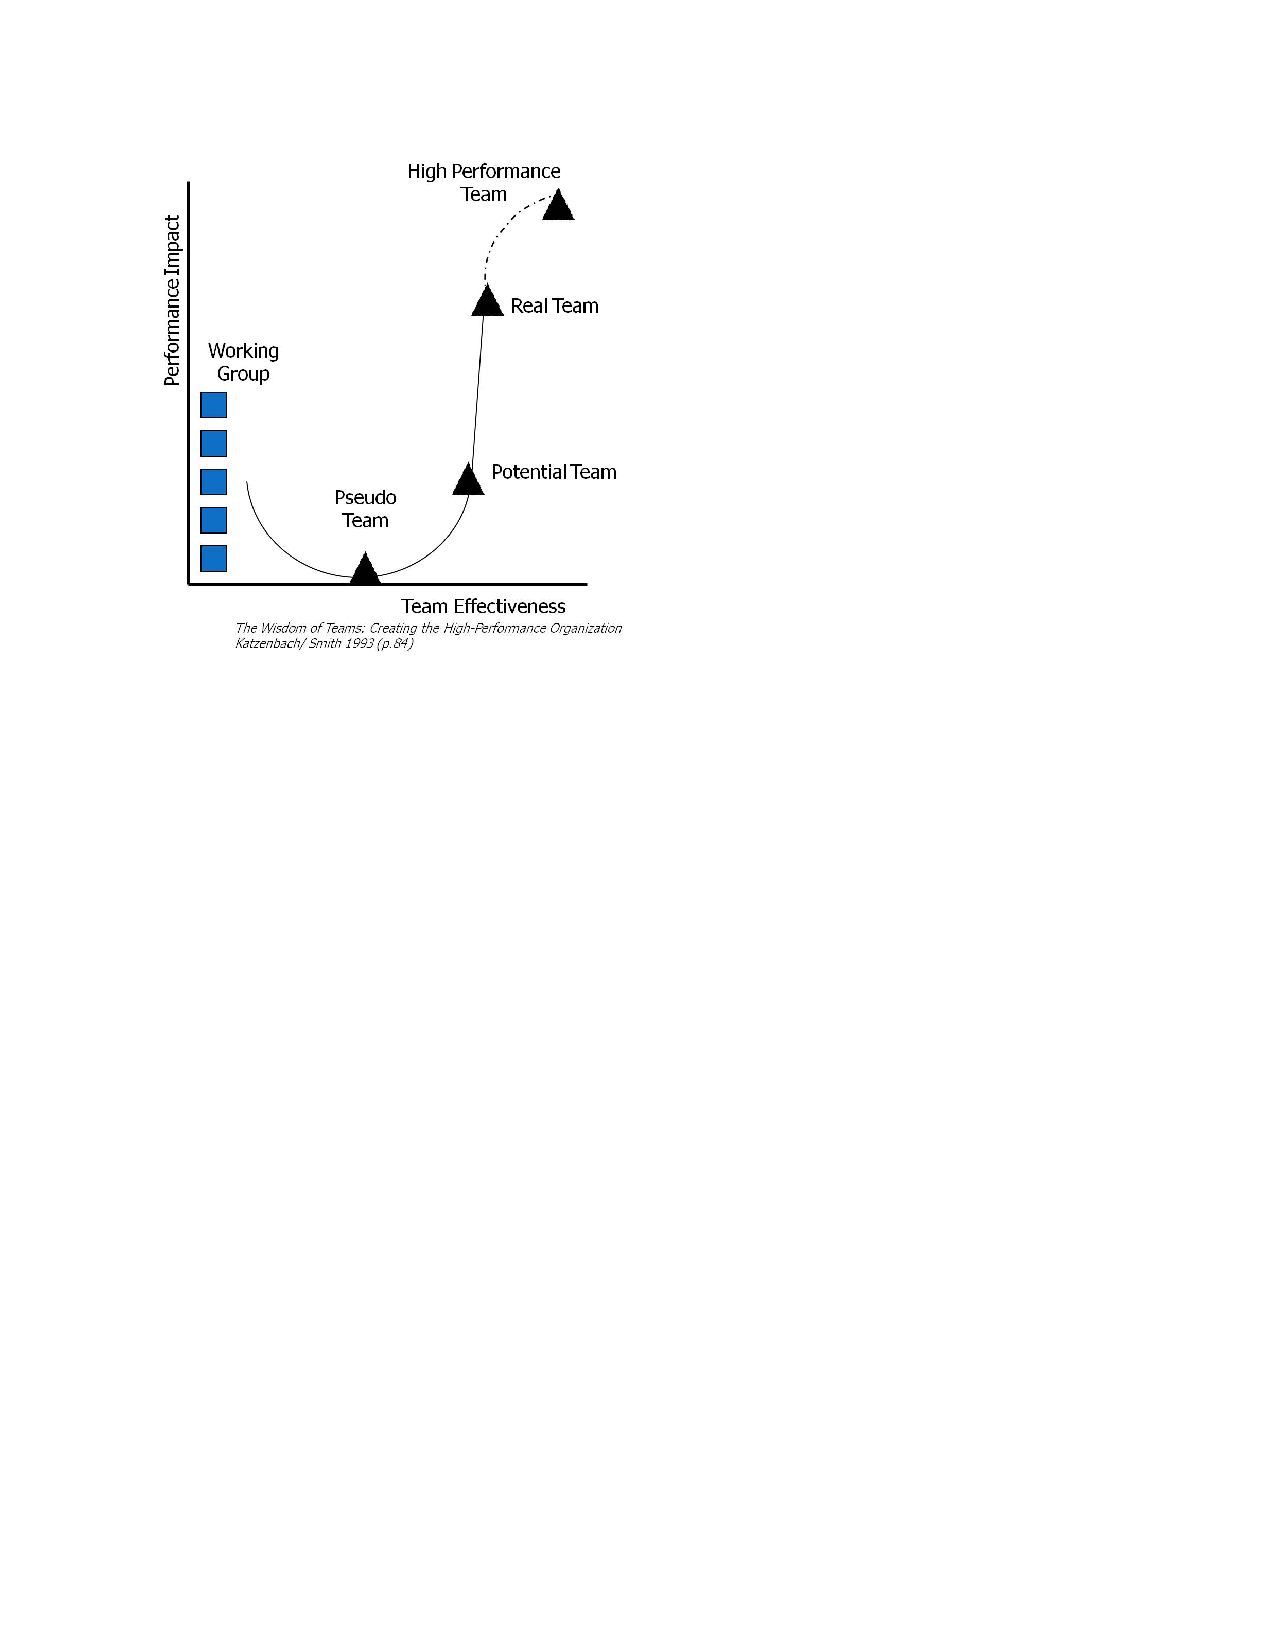
\includegraphics[clip=true, width=1 \textwidth,
trim=0cm 16cm 4cm 2cm]{Gruppetypene.pdf}
\captionof{figure}{De ulike gruppetypene}
\label{fig:gruppetype}
\end{center}

\end{enumerate}

Basert på disse karakteristikkene konkluderer vi med at vår gruppe kan karakteriseres som en effektiv gruppe. Vi er alle tilfredse og fornøyde med å arbeide sammen i en gruppe. Dessuten bidrar en felles karakter til gjensidig avhengighet og et insentiv for at alle bidrar for å oppnå et best mulig fellesresultat. Vi har regelmessige refleksjoner der vi vurderer vår egen fremdrift og effektivitet. Grunnet mangel på svært sterke emosjonelle bånd kan vi ikke definere oss som en ``high-performance''-gruppe selv om det er god stemning og vi alle etterstreber et best mulig fellesresultat. Det er ikke naturlig å forvente dette gruppetypenivået for vår gruppe da vi har svært begrenset med tid over en avgrenset tidsperiode på noen uker.\\

\section{Enighet}
\label{sec:enighet}
Enigheten i gruppa har generelt sett vært stor. Vi kan peke på flere faktorer som vi mener kan være årsaker til stor enighet innad i gruppa. I Schwarz (2002) \citep{fasilitator} sin tredje grunnregel for effektive grupper fokuseres det på at gruppemedlemmer må bruke spesifikke eksempler og bli enige om hva viktige ord og begreper betyr. Dette er et område vår gruppe har fokusert på fra første dag. Vi har vært svært opptatt av at alle har en felles forståelse av det vi diskuterer slik at man unngår misforståelser. Dette har vi oppnådd ved at alle parter, både formidler og mottaker av informasjon, til enhver tid har stilt spørsmål for å forsikre seg om at de forstår hverandre. I arbeid med utforming av tabeller til databasen hadde vi en situasjon mellom Mats og Linn som fint illustrerer dette poenget.\\

\textit{``Mats holdt på å skissere ER-diagrammet til databasen da Linn bryter inn: `det der blir vel snarere et klassediagram, jeg tror vi må gjøre det sånn her'. Linn starter å tegne sin versjon av ER-diagrammet på tavla. Mats følger litt forvirret med på Linns skisse og da hun har fått frem poenget spør han `hva er det egentlig som blir forskjellen, kan du forklare det litt nærmere Linn?' Linn forklarer hva hun mener slik at det ender med at begge er enige og oppnår en felles forståelse av de brukte ordene og begrepene.''}\\

Denne situasjonen bekrefter at det er viktig med oppklaringer underveis i diskusjoner for å bli enige på samme grunnlag. Dette fokuset har trolig medført at gruppa har opplevd større grad av enighet siden misforståelser er oppdaget på et tidlig tidspunkt.\\

Samarbeidsavtalen og like bakgrunner kan være andre årsaker til stor enighet i gruppa. Store deler av dag tre ble brukt til å skrive en samarbeidsavtale. I denne forbindelse var det mye diskusjoner om hva våre ambisjoner for faget var, og hvordan vi ønsket å jobbe. Gjennom denne diskusjonen ble ønskede arbeidsforhold dokumentert slik at disse punktene lå i underbevisstheten vår under hele arbeidsprosessen. Det er mulig å anta at dette kan ha påvirket enigheten i gruppa siden vi dannet en felles plattform for hvordan vi så for oss prosjektet. På denne måten baserer alle sine meninger til dels på allerede felles prinsipper. Det faktum at vi alle har relativt like bakgrunner med tanke på utdanning og alder bidrar nok også mye til stor enighet. Vi har alle en teknisk ingeniørbakgrunn og liker struktur og bestemte måter å jobbe på. Lik utdanning og alder bidrar også til at vi oppfatter problemer på samme måte, i tillegg til å ofte se de samme løsningene.\\

Enighet i gruppa er på mange måter positivt da man unngår ubehagelige problemer og konflikter, og arbeidsprosessen går smidig og uten store hindringer. Likevel kan for stor enighet medføre at man ikke oppnår det best mulige resultatet \citep{effectiveTeams}. Denne faren kan oppstå fordi gruppemedlemmer er redd for å skape uenigheter i en ellers samlet gruppa og dermed ødelegge en god atmosfære. Dette potensielle problemet har vi forsøkt å unngå ved å følge retningslinje seks presentert av Johnson \& Johnson (2013)\citep{gruppeteori} i ``Creating effective teams'': ``engasjer deg i konstruktiv kontrovers ved å være uenig og utfordre hverandres konklusjoner og resonnementer slik at kreativ beslutningstaking og problemløsning fremmes.'' Retningslinjen er fulgt ved at vi ved rask enighet har forsøkt å stille spørsmålstegn ved vår egen løsning, for eksempel ``hva er alternative løsninger?'' og ``hva er svakhetene ved vår løsning?''. Dette er en metode som har fungert relativt godt siden det har gitt diskusjonene nye dimensjoner og tvunget oss til å se saken fra ulike perspektiver.\\

\section{Involvering}
\label{sec:involvering}
Som nevnt tidligere i prosessrapporten består gruppa av både ekstroverte og introverte personer. Dette var noe vi identifiserte allerede på vår første sammenkomst. Det var lettere for enkeltpersoner å ta ordet og initiativ i forbindelse med diskusjoner og oppgaver. Wheelan (2009)\citep{effectiveTeams} påstår at kommunikasjonsmønstre etableres veldig raskt i en gruppeprosess. Hun snakker også om at effektiviteten og ytelsen til en gruppe kan lide når roller og involvering av medlemmer blir ignorert. Alle medlemmer må ta ansvar for å forsikre seg at andre blir hørt og er trygge med rolleinndelingen siden dette vil øke sjansen for gruppesuksess. Verdifulle innspill og ferdigheter vil da bli brukt istedenfor å gå tapt.\\

På landsbydag to observerte en av fasilitatorene blikkontakten blant medlemmene under en gruppediskusjon. Resultatet er vist i figur ~\ref{fig:sosiogram1}. Denne bekreftet antakelsen til gruppa om at det muligens var en skjevfordeling av deltakelse i diskusjonene.\\

\begin{center}
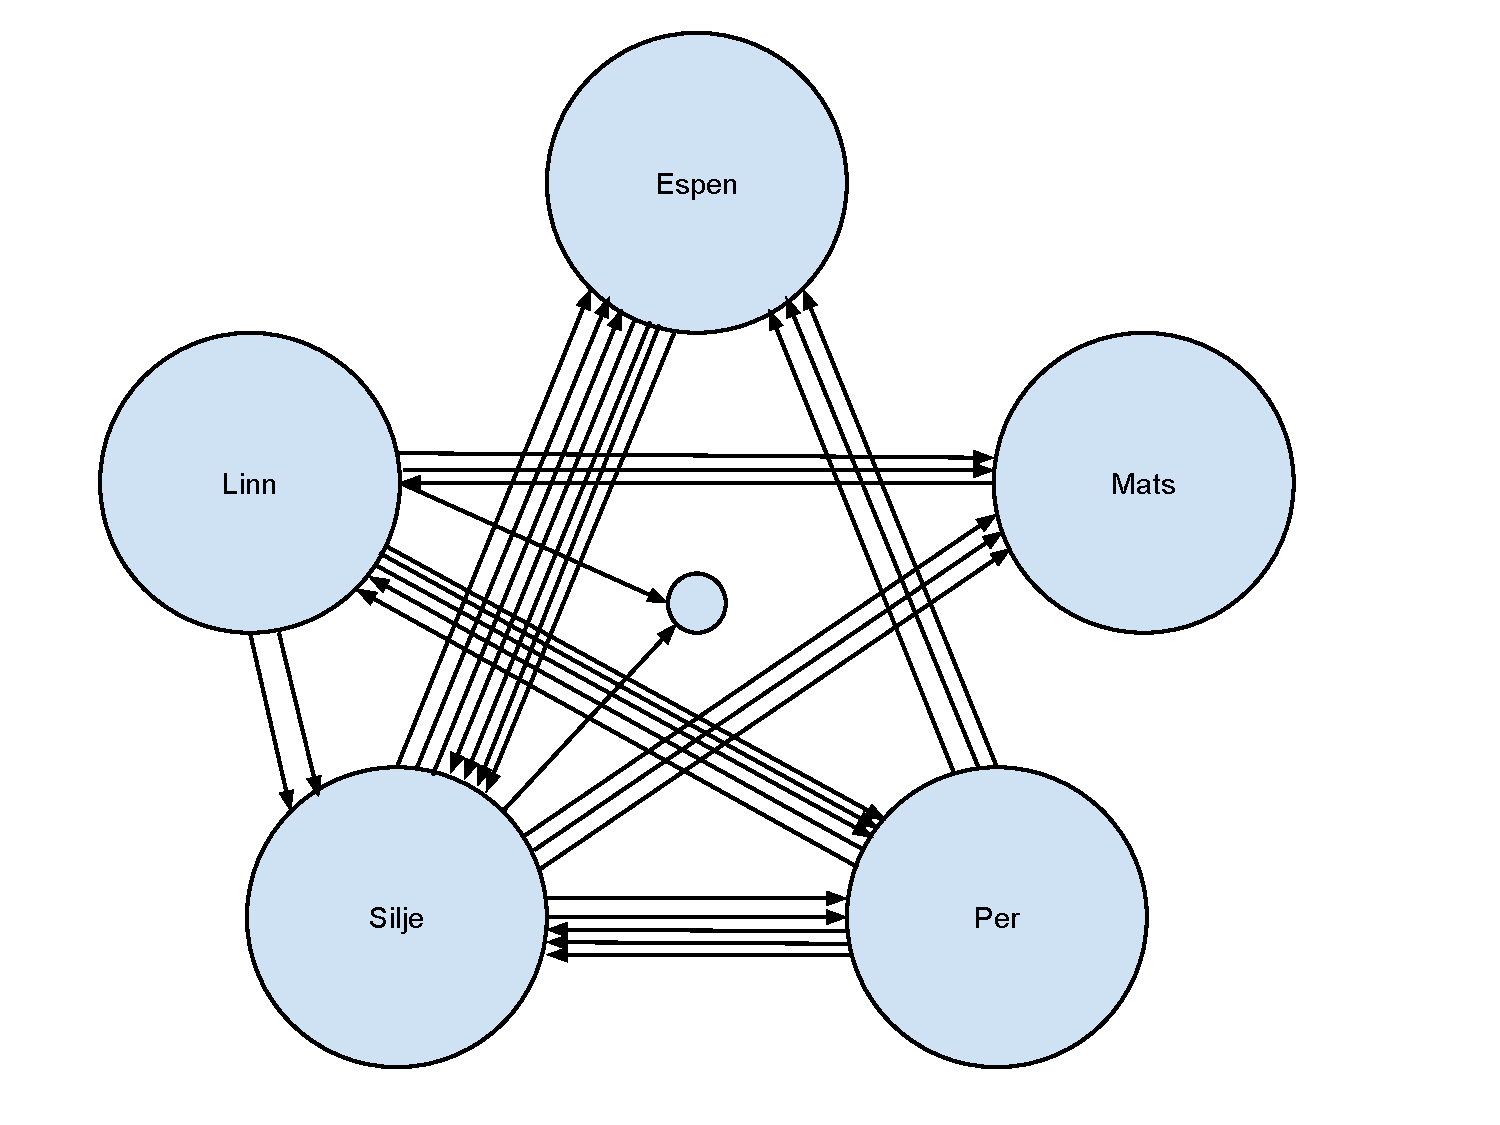
\includegraphics[clip=true, width=1 \textwidth,
trim=0cm 0cm 0cm 0cm]{Sosiogram1.pdf}
\captionof{figure}{Sosiogram 1}
\label{fig:sosiogram1}
\end{center}

I sosiogrammet over ser vi en tendens til at enkeltpersoner er mindre involvert. Man ser også antydninger til dominans fra enkeltindivider ved at mye blikkontakt er rettet mot disse. En av begrunnelsene for dette kan være at noen tar initiativet mer enn andre slik at mye fokus blir rettet mot disse personene. Et annet viktig punkt som kommer fram er at mindre fokus må rettes mot enkeltpersoner. Henvendelser må heller rettes mot hele gruppa i drøftinger. For å skape variasjon i blikkontakten i diskusjonene valgte derfor gruppa å endre sitteposisjonene seg i mellom ved jevne mellomrom. Vi håpet at dette skulle åpne opp for å lettere komme i blikkontakt med alle gruppemedlemmene i løpet av diskusjonene. Det var også viktig at alle ble observante på dilemmaet, og gjorde sitt beste for å inkludere de andre medlemmene, spesielt de som syns det er vanskeligere å ta ordet.\\

Etter de to første landsbydagene prøvde vi å sette aksjonene våre ut i praksis for å se om vi klarte å skape en plattform for deltakelse og involvering. Under arbeidet med å finne en problemstilling til prosjektet utførte vi en brainstormingprosess. Det virket som at det var en lav terskel for å komme med innspill, og vi så en omtrentlig jevn fordeling av bidragene. Espen, Linn og Silje var fortsatt partene som tok initiativet, men både Mats og Per var mer delaktige i diskusjonene. Gruppa ble enig om at det er viktig at initiativtakerne retter spørsmål og spørrende blikk mot de mer introverte partene. Dette samsvarer med Wheelan (2009)\citep{effectiveTeams} sin betraktning om at å forsikre alle sin deltakelse kan være så enkelt som å stoppe periodisk opp for å høre med alle.\\

Etter valg av tema for prosjektoppgaven skulle gruppa utarbeide en detaljert problemstilling. I den anledning foreslo Espen en uortodoks metode der hvert medlem måtte komme med et ord om gangen og dette gikk på rundgang til en fullstending problemstilling var ferdig. Dette viste seg å være en morsom og enkel måte å få alle medlemmene delaktige. Problemstillingen som ble utarbeidet viste seg også å være relativt lik den som ble brukt i selve prosjektet, noe som viste at en felles forståelse av problemet hadde blitt oppnådd ved den gode diskusjonen i brainstormingsprosessen.\\

En annen ting som ble tydelig denne dagen var at digresjoner var nyttige for å skape trygghet og trivsel i gruppa. Gruppa påpekte at det er viktig at disse digresjonene ikke tar overhånd, men at litt digresjoner skaper åpenhet innad i gruppa. Videre observerte flere at Per virket generelt mer deltakende i diskusjonene, og gruppa lurte på om dette kunne være på grunn av de tidligere aksjonene. Det var vanskelig å konkludere med at aksjonene allerede var vellykket, men gruppen valgte å se på det som et steg i riktig retning og ville fortsette med å skape en arbeidsplass hvor inkludering og trygghet var i fokus.\\

På landsbydag fire bestemte gruppa seg for å ha en overordnet rolleinndeling. I diskusjon rundt rollene virket både Mats og Per usikre på hvilken rolle de ville besitte. I den anledning bestemte Linn seg for å sette begge ovenfor et dilemma. I dette dilemmaet måtte de velge en spesifikk rolle. Dette var en god form for inkludering og skapte en sunn diskusjon som virket å skape ytterligere åpenhet mellom gruppemedlemmene. Vi ble enige om at å stille hypotetiske spørsmål kunne være en smart aksjon for å fremtvinge diskusjoner og skulle etterstrebes i høy grad.\\

Som nevnt tidligere hadde Per vist tegn til å ha følt en større trygghet i landsbydag tre, mens Mats enda hadde forholdt seg relativt stille. I landsbydag fem oppsto det dog en situasjon der Mats trådde frem. I en diskusjon rundt databasen tok han initiativ og stilte en rekke spørsmål. Det er nok flere faktorer som har innspill i denne situasjonen, eksempelvis at han føler seg mer komfortabel med å diskutere aspekter han har kunnskaper innenfor, men vi tror også at dette har med de tidligere nevnte aksjonene. De introverte gruppemedlemmene blir mer og mer delaktige, og gruppen ser en progresjon i samhold og effektivitet.\\

Et annet viktig punkt som ble observert var at enkelte av de ekstroverte personene virket å være mer observante på sin adferd. I diskusjoner prøvde disse å forholde seg mer passive for å åpne opp for at andre kunne ta initiativ og ordet. Dette er enda et tegn på gruppemedlemmenes villighet til å strebe etter et velfungerende og effektivt team gjennom inkludering.\\

I neste landsbydag jobbet Mats og Per med prototypen. I den anledning oppsto det et spørsmål vedrørende designet. Mats valgte da å forhøre seg med Silje for å få råd og meninger. Først og fremst var dette enda et tegn på at plattformen for åpenhet og inkludering vi hadde prøvd å skape virket å være vellykket. Wheelan (2009)\citep{effectiveTeams} nevner at hvis man skal dra nytte av mangfold i grupper så må alle bli involvert og hørt i diskusjoner. Selv om gruppa jobber i to subgrupper (programmering og rapportering) så er det mulig å stille spørsmål på tvers av subgruppene. En annen interessant ting var at det var en av de introverte personene som startet denne diskusjonen gjennom en rådgivning. Dette så vi på som et meget positivt tegn i forhold til oppnåelse av trygghet i gruppa.\\

Ved landsbydag åtte ble gruppa fasilitert i en av diskusjonene. Her ble diskusjon mellom de ulike partene fremstilt i et sosiogram som er illustrert i figur ~\ref{fig:sosiogram2} nedenfor. Det er viktig å poengtere at dette sosiogrammet ikke tar for seg eksakt det samme som sosiogrammet tidligere i dette delkapittelet, men omhandler i det store bildet det samme. Essensen er at begge får frem involvering i ulike diskusjoner. Det nye sosiogrammet viser helt klart forbedringer i gruppa, og vi ser en mer jevn fordeling av deltakelse. Et viktig aspekt er at både Mats og Per ikke bare henvender seg  til enkeltpersoner, men tar opp diskusjoner i hele gruppa. Det viser igjen at de introverte personene føler en større trygghet, og til og med er med på å skape involveringen selv.\\

\begin{center}
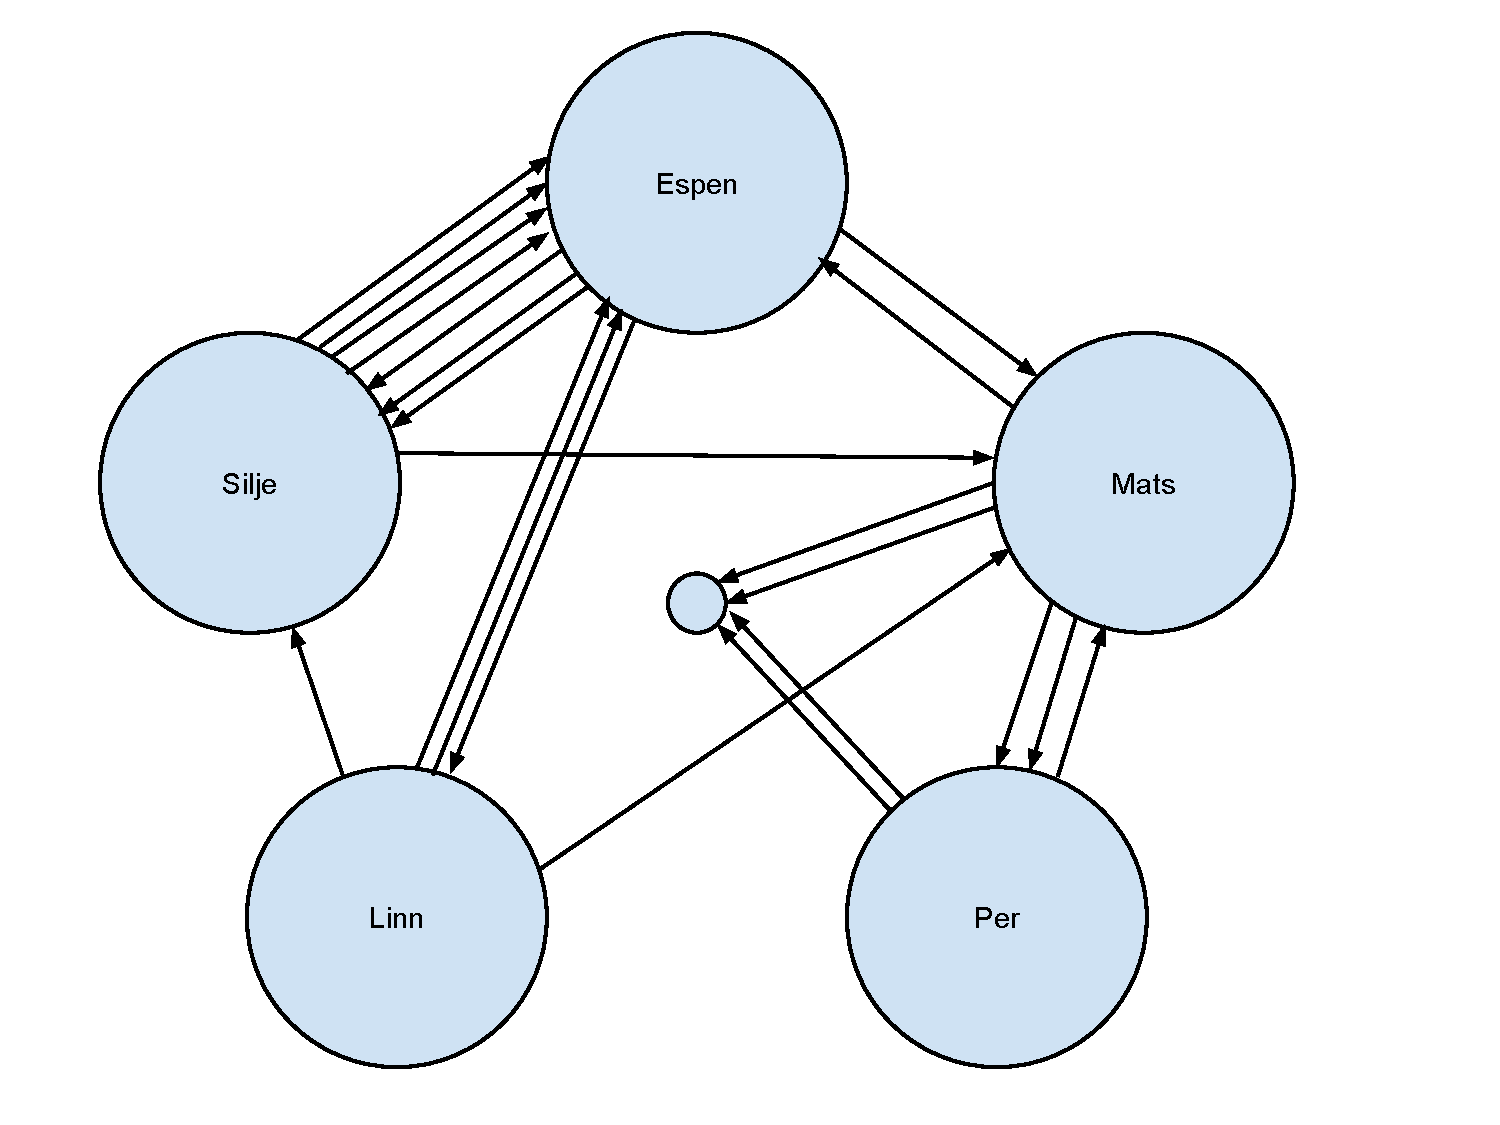
\includegraphics[clip=true, width=1 \textwidth,
trim=0cm 0cm 0cm 0cm]{Sosiogram2.pdf}
\captionof{figure}{Sosiogram 2}
\label{fig:sosiogram2}
\end{center}

En annen situasjon som oppsto på dag åtte var at Silje ved morgenmøtet lot være å ta initiativet for å gi andre muligheten. Det tyder på at de mer dominerende partene faktisk er observante på sin egen oppførsel, og er villige til å ta tak for å fremtvinge andres deltakelse.\\

I neste landsbydag kommenterte en av fasilitatorene kroppsspråket til deltakerne i en diskusjon. Han påpekte at alle var fremoverlente. En slik kroppsholdning i diskusjoner kan gjerne tyde på engasjement, og at deltakerne vil bidra med sine innspill, samtidig som de får med seg andres poenger. Observasjonen tyder på at medlemmene føler seg trygge på hverandre, og ikke er redde for å stille seg i skuddlinjen. Det er viktig at slike felles gruppediskusjoner blir brukt så ofte som mulig siden de er et godt verktøy for å videre utvikle både gruppemedlemmene på et personlig plan og gruppa som helhet.\\

Den kommende landsbydagen brakte med seg en diskusjon rundt koblingsagenten når det daglige statusmøtet ved lunsj ble utført. Fasilitatoren påpekte at alle gruppemedlemmene var delaktige i diskusjonen, og at bidragene var jevnt fordelte. Det er viktig at disse gruppediskusjonene forsetter som nevnt tidligere. Dette har ikke bare med involvering å gjøre, men også for å kunne benytte alles egenskaper og kunnskaper, samtidig som at de ulike medlemmene føler et eierskap til alle deler av prosjektet.\\

I løpet av avslutningsfasen av prosjektet så vi flere tegn på at gruppa hadde lyktes i sitt forsøk på å involvere alle i gruppa. Vi har valgt å trekke fram en spesifikk episode som vi føler gir en god indikator på dette. Ved landsbydag 11 valgte Mats å ta initiativet til oppstarten av det daglige statusmøtet etter lunsj. I en tidligere fase av prosjektet ville det vært ganske utenkelig at en av de introverte partene hadde stilt seg selv i skuddlinja, og vi anser derfor våre aksjoner som vellykkede. Alt i alt har involveringen både vært viktig for gruppas utvikling, men også for den personlige utviklingen til de ulike medlemmene.\\


\section{Beslutningstaking}
\label{sec:beslutningstaking}
I sin gruppeeffektiviseringsmodell presenterer Schwarz (2002)\citep{fasilitator} tre faktorer som bidrar til høy gruppeeffektivitet: gruppeprosessen, gruppestrukturen og gruppekonteksten. Et av punktene diskutert under gruppeprosess er beslutningstaking. I en effektiv beslutningstakingsprosess er det flere mennesker involvert . Det eksisterer en rekke beslutningstakingmetoder: konsultativ (lederen bestemmer  ved å konsultere resten av gruppa), delegerende (lederen delegerer beslutningstakingen til andre medlemmer), konsensus (beslutning oppnås når alle medlemmer kan støtte beslutningen) og demokratisk (avstemming ved flertall). Kjerneverdier ved fasilitering påstår at en gruppe er mer effektiv dersom gruppa er internt forpliktet til valgene de tar \citep{fasilitator}.\\

Basert på denne forskningen har vår gruppe valgt å strebe etter konsensus i alle beslutningstakinger, men der dette ikke lar seg gjøre skal beslutningen tas ved flertallsavstemming. Som nevnt i \ref{sec:gruppesammensetning} har vår gruppe vært preget av en stor grad av enighet slik at det stort sett har gått greit å oppnå konsensus. I beslutningen forbundet med valg av problemstilling ble konsensus vellykket gjennomført.\\

\textit{``I arbeidet med problemstillingen startet vi med brainstorming med høy grad av involvering av alle medlemmene. Deretter gikk vi gjennom hvert forslag hvor alle sa ja eller nei, ja-forslagene ble beholdt, mens nei-forslagene ble forkastet. Resultatet ble tre ideer; koblingsagent, intelligente systemer og eVoting som vi tok en inngående diskusjon av. Det ble tydelig under diskusjonen at Espen, Linn, Silje og Mats hellet i retning av koblingsagent. Per derimot var mest gira på intelligente systemer. Han fortalte at dette var et tema som interesserte han mer, og som han allerede hadde en del kunnskap om. Espen tok deretter ordet for å påpeke fordeler med å velge koblingsagenten. Han fokuserte på at vi lettere kunne benytte alle medlemmenes kunnskaper i forbindelse med en koblingsagent, i tillegg til at kompleksiteten på oppgaven var mer passende vårt tidsperspektiv. Etter litt videre diskusjon om disse faktorene, ble Per stadig mer overbevist om at koblingsagenten var et valg som ville være bra for gruppa som helhet. Vi landet derfor på en problemstilling som alle kunne stille seg bak og var motiverte for å jobbe med.''}\\

Denne situasjonen ga gruppa en positiv opplevelse av konsensusmetoden. Vi erfarte at en dyptgående gjennomgang medførte at alle fikk komme med sitt syn, samtidig som gode argumenter ble presentert slik at vi dannet en felles forståelse. Dessuten unngikk vi personangrep, og diskusjonen ble drevet videre av saklige argumenter. Alle disse poengene har ligget i underbevisstheten vår i det videre prosjektarbeidet. Dette, i tillegg til at konsensus som primær beslutningsmetode ble nevnt i samarbeidsavtalen, kan ses på som aksjoner vi har gjennomført for å fortsette den gode opplevelsen av konsensusmetoden i beslutningssituasjoner.\\


\section{Samarbeidsindikator}
\label{sec:samarbeidsindikator}
%FIX X OG XX
I løpet av prosjektfasen ble det avholdt to relativt like spørreundersøkelser, henholdsvis på dag fem og ti. Disse førte med seg en samarbeidsindikator hver illustrert som pentagram i appendix \ref{appendix:samarbeidsindikator1} og \ref{appendix:samarbeidsindikator2}. Det er viktig å poengtere at den første spørreundersøkelsen ble utført av alle fem gruppemedlemmene, mens den andre bare ble gjennomført av fire slik at resultatene ikke kan sammenlignes med fullstendig nøyaktighet. Pentagrammene fremstiller fem kategorier av samarbeid, og disse vil bli videre reflektert over i avsnittet.\\

Den første kategorien omhandler i hvilken grad gruppas medlemmer forholder seg til hverandre på et personlig og direkte plan. Schwarz (2002)\citep{fasilitator} får frem at det er viktig at medlemmer er direkte med hverandre, og ikke trenger å bruke en mellommann, for å forsikre seg om at at meningene deres blir oppfattet som tilsiktet. Han nevner videre at gruppemedlemmer må kunne uttrykke seg personlig og direkte uansett hvilken posisjon eller status de har i gruppa. Hvis vi ser på samarbeidsindikatorene kan man se en minimal forbedring, og ligger ikke i en faresone.\\

Det andre feltet fokuserer på hvordan gruppa forholder seg til hverandre og det som skjer innad. Johnson \& Johnson (2013)\citep{gruppeteori} diskuterer fire ulike gruppetyper. I avsnitt \ref{sec:gruppetype} konkluderer vi med at gruppen vår tilhører kategorien ``effektive grupper''. Dette kommer mye av at man føler en gjensidig avhengighet av hverandre, og er fokusert på å være oppdatert på andres arbeid. Dette blir også gjenspeilt i bruken av statusmøter i løpet av arbeidsdagene. I pentagrammene ser vi en forbedring på dette punktet. En av årsakene kan være innføringen av de nevnte statusmøtene.\\

I den tredje kategorien blir graden av snillhet og forsiktighet mellom gruppas medlemmer fremstilt. I følge pentagrammet ser vi en kraftig tilbakegang på dette punktet, og ligger i området for en stor utfordring. En av karakteristikkene ved samarbeidsgrupper er mer effektiv kommunikasjon og en vennligere atmosfære \citep{fasilitator}. Dette er en av grunnene til at vi mener det nødvendigvis ikke trenger å være direkte negativt at gruppen har skapt en mer vennlig atmosfære, og at dette kan ha bidratt til å oppnå en mer effektiv gruppe. Wheelan (2009)\citep{effectiveTeams} nevner også en vennligere gruppeatmosfære som et positivt punkt, og trekker videre fram konformitet som et positivt aspekt for samhold i grupper, noe som en vennligere atmosfære kan føre med seg.\\

Det fjerde aspektet samarbeidsindikatorene tar for seg er i hvilken grad gruppa er preget av lite struktur og svak disiplin. Schwarz (2002)\citep{fasilitator} lister opp åtte punkter som er viktige for en god gruppestruktur. Mange av disse omhandler måloppnåelse og visjoner, noe som vår gruppe har sett store likheter innenfor. Det er derfor ikke overraskende at pentagrammene viser at gruppa ikke ligger i faresonen.\\

% sjekke avsnitt 2.2.. om det er riktig referanse.
Den siste kategorien omhandler gruppas grad av asymmetri og isolasjon. Dette er noe som har blitt reflektert over flere steder i prosessrapporten (spesielt avsnitt 2.2), og har vært et stort fokus for gruppa. Samarbeidsindikatorene viser at vi plasserer oss på samme sted i pentagrammene begge ganger. Etter en refleksjon mellom gruppas medlemmer virket det veldig naturlig at vi blir plassert såpass langt ut på skalaen, men føler ikke at det trenger å være en stor utfordring. Gruppa har vært observante på fenomenet fra oppstarten, og har prøvd å snu asymetrien til en styrke der de introverte og ekstroverte partene får brukt alle sine egenskaper.\\


\section{Utvikling i løpet av prosjektperioden}
\label{sec:utvikling}
I gruppedynamikk snakker man gjerne om Tuckman sine stadier for gruppeutvikling. Denne teorien diskuterer fire spesifikke faser som er nødvendig for en gruppe for å oppnå fremgang og for å ta tak i utfordringer på en god måte. Disse fire fasene er: ``Forming'', ``Storming'', ``Norming'' og ``Performing''. Vi har valgt å ta utgangspunkt i denne teorien for å fremstille vår utvikling i løpet av prosjektfasen. De ulike fasene er illustrert i figur ~\ref{fig:faserigruppesamarbeid} under.\\

\begin{center}
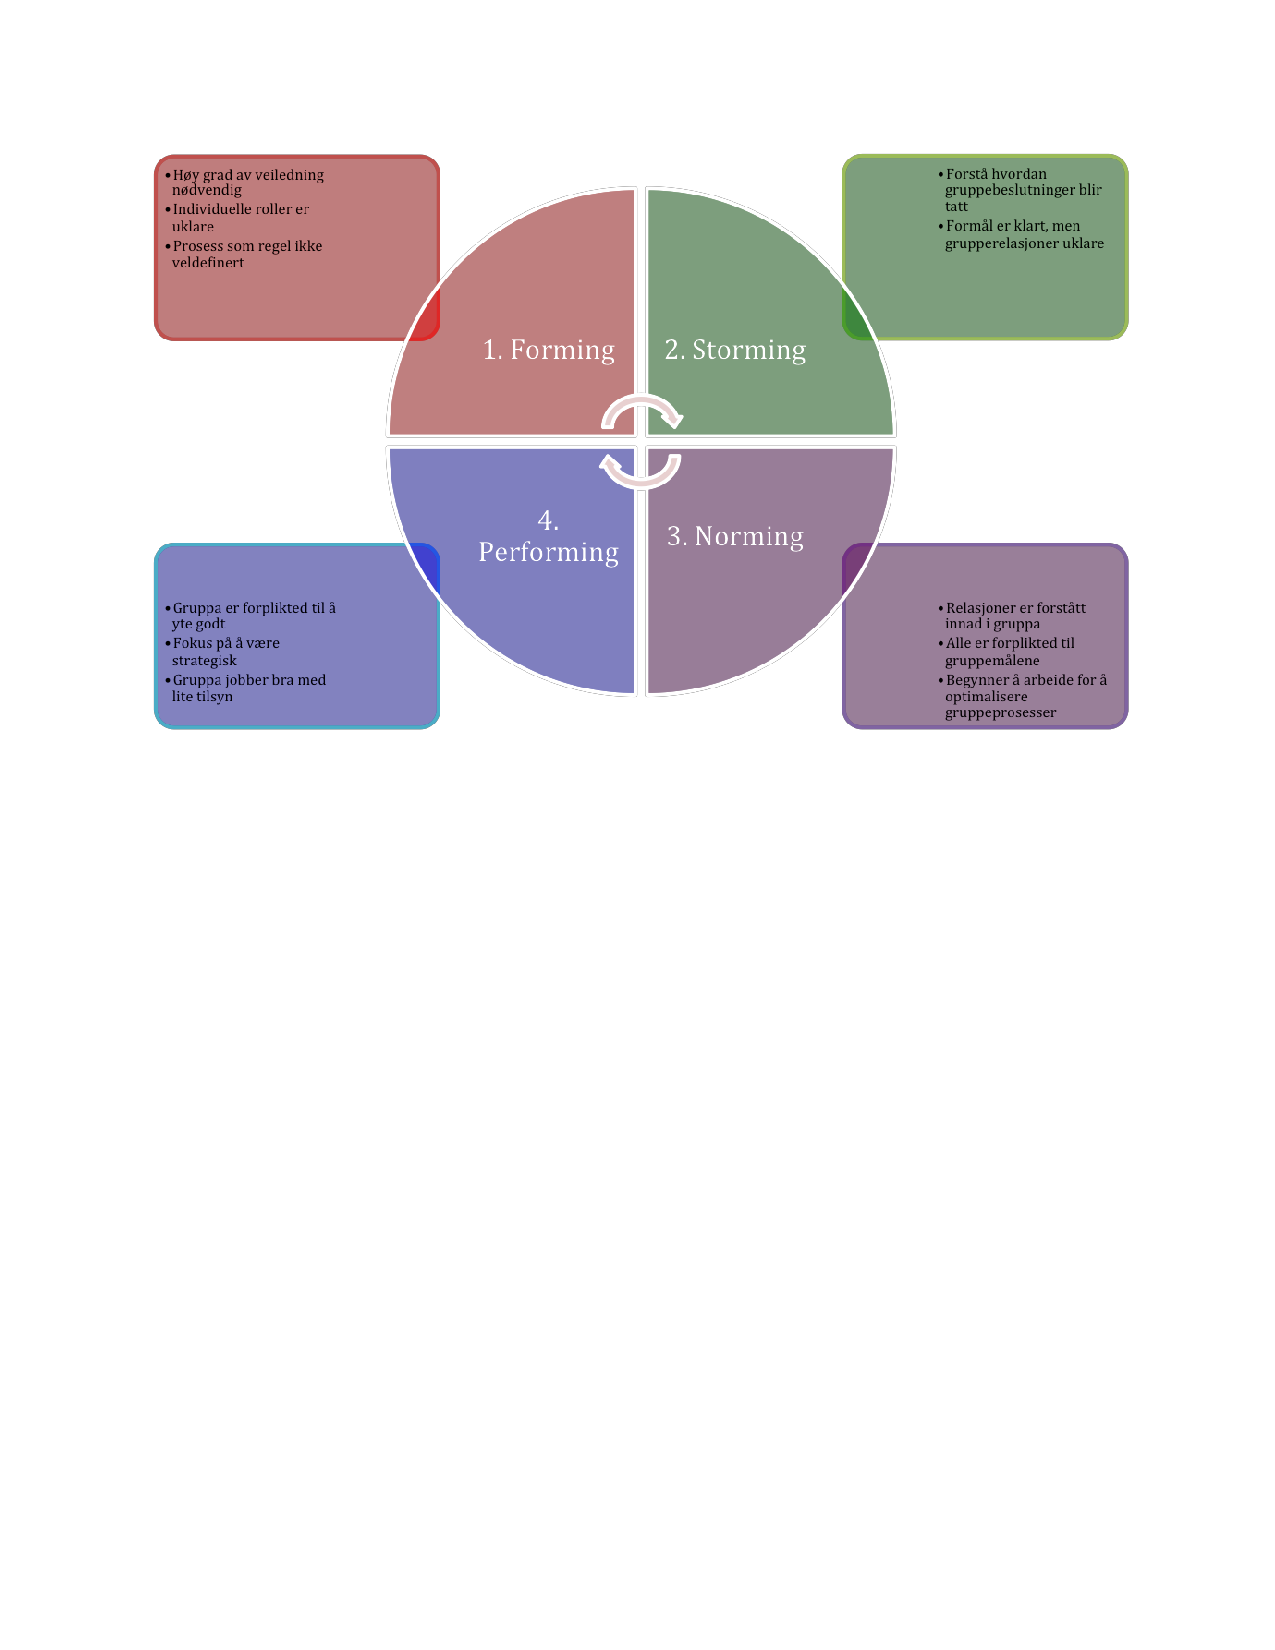
\includegraphics[scale=0.9,
trim=2.7cm 14cm 0cm 5cm]{Faserigruppesamarbeid.pdf}
\captionof{figure}{Tuckmans faser i gruppesamarbeid}
\label{fig:faserigruppesamarbeid}
\end{center}

I ``forming'' fasen skal gruppemedlemmene bli kjent med hverandre. Problemer som organisering og rolleinndeling er tatt hånd om her. En annen ting som blir satt i søkelyset i denne fasen er hvordan de ulike personene arbeider individuelt, som et gruppemedlem, og hvordan de tåler press. Dette var alle faktorer som ble synlige i oppstarten av prosjektet i form av øvelsene hvor vi skulle utarbeide en kompetansetrekant og gjøre gruppa bevisst på gode og dårlige sider ved deg selv.\\

Når man avanserer fra ``forming'' stadiet skal man i teorien entre ``storming'' fasen. Dette var noe som ikke var like tydelig i gruppa vår. Her er det naturlig at gruppemedlemmene reflekterer og kommuniserer over sine syn, og diskusjoner blir ofte utført. Gruppa føler denne fasen omtrent ble neglisjert. Enighet rundt eksempelvis hvordan gruppebeslutninger skulle tas gikk hurtig og smertefritt.\\

``Storming'' fasen var som sagt relativt kort, og ledet opp til ``norming'' stadiet. I denne fasen vokste gruppa til en velfungerende enhet. Et viktig aspekt var at gruppa utarbeidet en felles plan, samtidig som felles mål og ambisjoner ble veldefinerte og fastsatt.\\

Den fjerde og siste fasen er kalt ``performing'' stadiet. Det er viktig å poengtere at ikke alle grupper klarer å oppnå et slikt nivå av gruppeutvikling og gruppedynamikk. Dette er gjerne omtalt som den hellige gral i forhold til gruppeprogresjon. Gruppemedlemmene følte at vi tidlig i prosjektfasen gikk inn i denne fasen. Mye av begrunnelsen var basert på etableringen av den felles planen, målene og ambisjonene. Gruppa hadde i den anledning på et tidlig stadiet fastsatt rammene for prosjektet, og gikk dermed på skinner. En annen viktig faktor for oppnåelsen av ``performing'' fasen var måten gruppa inndelte arbeidet der alle medlemmene fikk benyttet sine styrker. Effektivitetsnivået var meget høyt, som vi så på som et tegn for hvor langt gruppa hadde kommet som en enhet.\\

Som det fremgår av teksten over har gruppa faktisk gått gjennom de ulike stadiene i Tuckman sin teori om gruppeutvikling, men har omtrent forbigått ``storming'' fasen. Gruppa utviklet seg til en velfungerende enhet i løpet av prosjektet. Dette kunne observeres fra flere faktorer. Eksempelvis så man en stadig økning i produksjonsnivå og effektivitet. Det var en enighet om at oppnåelsen av denne fasen var meget positiv, spesielt siden dette ikke skal tas forgitt. Det er også viktig å ta i betrakning tidsaspektet og at gruppemedlemmene hadde liten kjennskap til hverandre på forhånd.\\
